%%%--------------------------------%%%
%%% Implementation
%%%--------------------------------%%%

\section{Gamification Elements}
\label{sec:implementationGami}

Though technically not necessary for the core functionality of risk management we decided to incorporate several gamification features and use cases into the \ac{MVP}. We proposed gamification as a possible means to adress the problem of negligence during project lifetime and consider the approach as the core contribution of this paper. Hence we gave gamification priority over several risk managment features as described above. The following will discuss the features we selected and our reasoning for doing so.

\begin{wrapfigure}{r}{0.5\textwidth}
	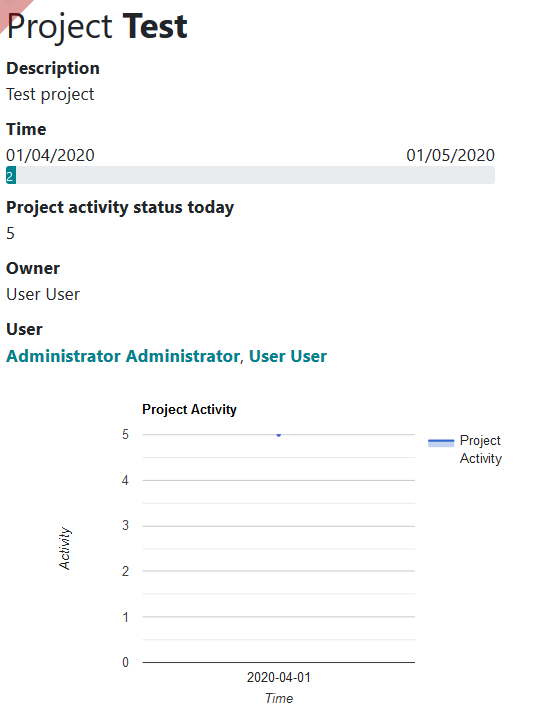
\includegraphics[width=0.5\textwidth]{Assets/implementation_shots/projectdetail.png}
	\caption{Screenshot showing progress visualizations}
	\label{fig:projectdetail}
\end{wrapfigure}

Besides achievements as shown in section \ref{sec:implementationInfra}, the \ac{MVP} has various further progress indicators which are part of the defined use case (\ref{sec:domainBbl}). First of all, users do receive points for desired behavior which can be seen in form of an activity graph for a single specific user or as an overall project activity, secondly the project detail view shows a progress bar based on the projects temporal progress. Both can be seen in figure XXX. This was realized because in addition to the motivational aspect the features can be seen as an indicator of project health which the reviewing project managers specificially requested (\ref{sec:DomainAb}).

Another approach to support the progress of a project is the implementation of a so-called task queue. To be specific, a user gets displayed further actions which make sense to continue working on after completing another task. One place where the application makes use of this is after proposing a project risk where options to propose another, review or discuss project risks are being displayed. The task queue, development wise, are simply links to different views of the application instead of more complex business logic. We consider this a very direct and low-threshold way to promote more user activity with the additional benefit of offering some explanation of the application functionalities.

Also, as part of the gamification elements and part of the defined use cases (\ref{sec:domainBbk}), an activity stream has been implemented. The application can keep track of events that occur during run time like the proposal of a new project risk. The activity stream can be found on the start page when logged in. An option to enable notifications is placed next to the activity stream which the user can use to allow its client to send notifications. Those notifications can be used in different use cases to inform the user about new events and make the application re-engageable (\ref{sec:theorieCa}). This is more of a core functionality than just gamification use case because it helps project members to stay on top of events and for those who dislike push notifications it covers the re-engagabilty of the application. It also provides entry points or shortcuts to different sections of the application.

\begin{figure}[H]
	\centering
	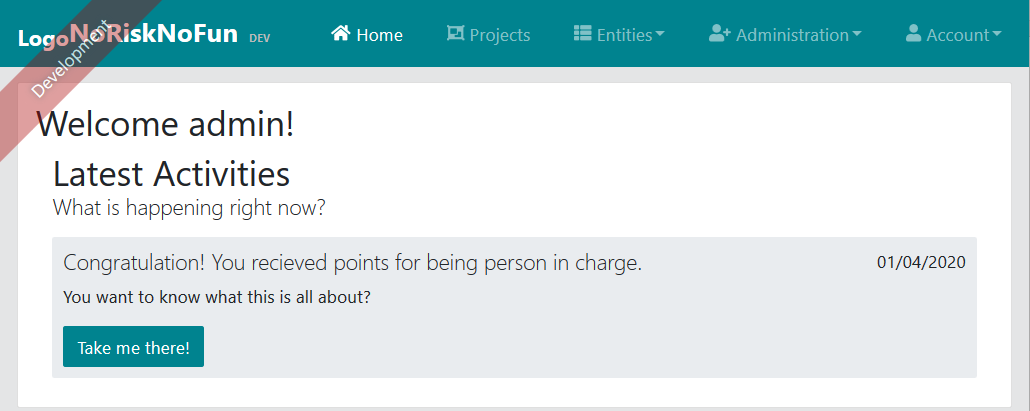
\includegraphics[width=0.8\textwidth]{Assets/implementation_shots/activitystream.png}
	\caption{Screenshot home screen with activities}
	\label{fig:activitystream}
\end{figure}

Not implemented is the use case Project Initialization (\ref{sec:domainBbj}) which is designed to encourage project members to create the first risks within a project. The reason this use case is not implemented is that it was considered lower priority because the inital risk estimation is less frequently neglected as the continuous management process (\ref{sec:theorieAc}).
Summarized, the following mechanics are realized as described the Gamification conception (\ref{sec:domainCc}) are part of the application: Activity Stream and Notifications, Badges, Praise and Rewards, Task Queues.